% C10. Semáforo de compra y recomendación
\begin{frame}{¿Compraríamos? Sí, como filtro y punto de partida, no como precio automático}
  \begin{columns}[c]
    \begin{column}{0.48\textwidth}\centering
      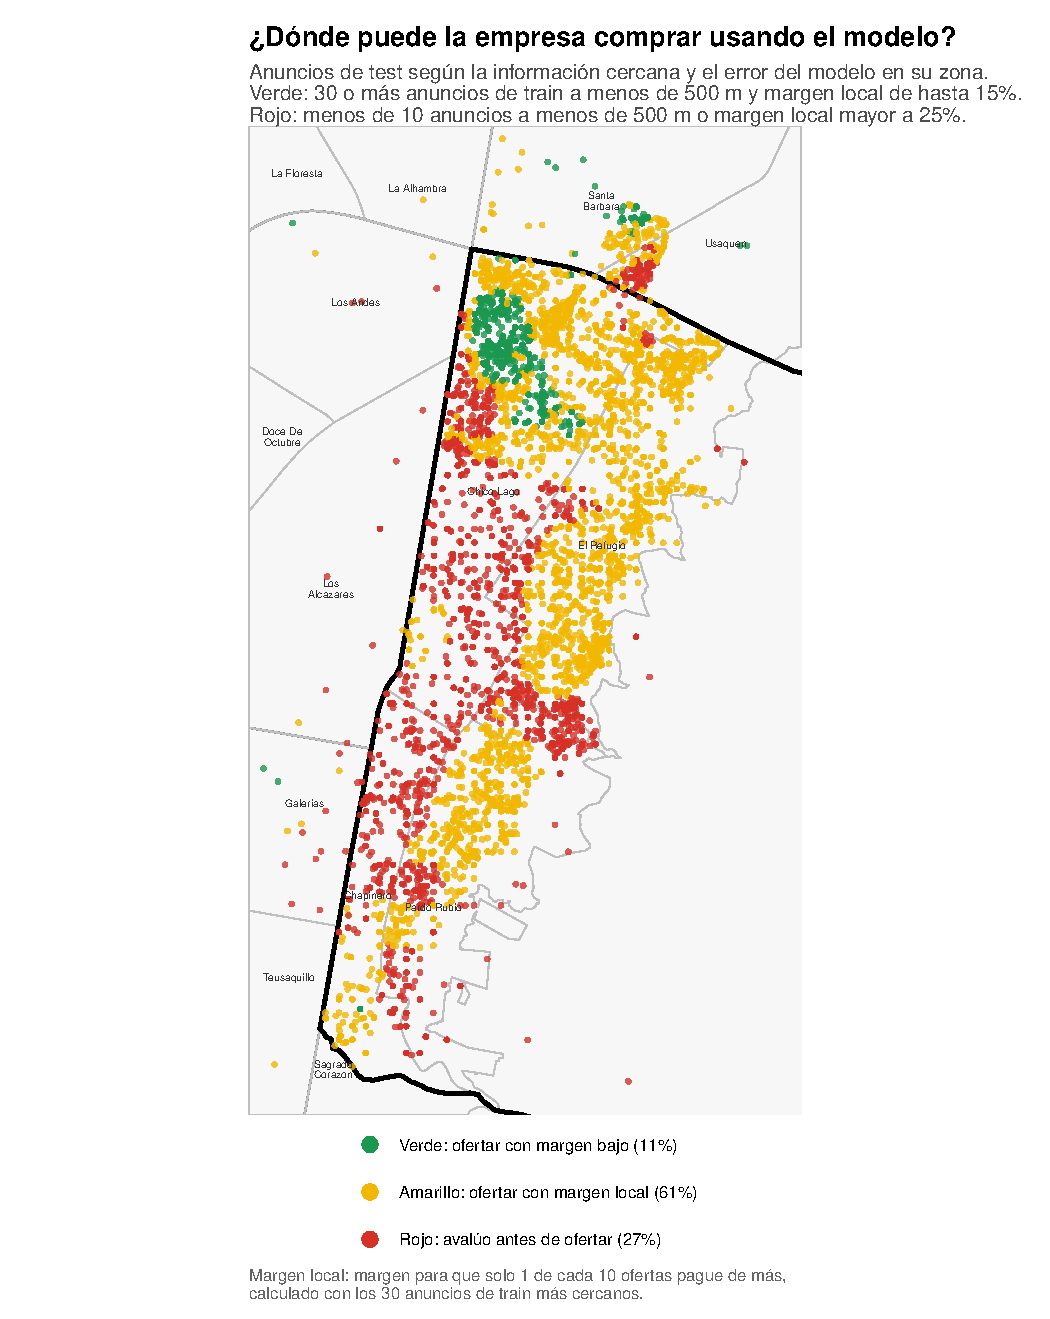
\includegraphics[height=0.84\textheight]{negocio_03_semaforo_test.pdf}
    \end{column}
    \begin{column}{0.5\textwidth}
      \textbf{\color{azul}Recomendación}
      \begin{enumerate}\small
        \item Usar la predicción como valor de referencia y ofertar alrededor de \margenchap{} por debajo.
        \item Verde (\pctverde): ofertar con margen bajo.
        \item Amarillo (\pctamarillo): ofertar con el margen de la zona.
        \item Rojo (\pctrojo): avalúo antes de ofertar.
        \item Monitorear las compras y reentrenar con los precios reales.
      \end{enumerate}
      \vspace{0.3em}
      {\small\color{gris}Riesgo principal: el vendedor acepta justo cuando el modelo le sobreestima la vivienda.}
    \end{column}
  \end{columns}
  \note{El semáforo combina dos cosas: cuántos anuncios de train hay cerca (si hay información) y qué tanto se equivoca el modelo en esa zona. El margen de \margenchap{} hace que solo 1 de cada 10 compras en Chapinero pague más que el precio. La compra automática no es rentable si el vendedor cede poco: los que aceptan son los que el modelo sobrevalora.}
\end{frame}
